% !TEX program = xelatex
% UTF-8 source. Compile in this directory with:
% xelatex -interaction=nonstopmode -halt-on-error seedvig_ei_reviewer_revised.tex
\documentclass[UTF8,a4paper,11pt,fontset=windows]{ctexart}

\usepackage[left=2.3cm,right=2.3cm,top=2.2cm,bottom=2.2cm]{geometry}
\usepackage{amsmath,amssymb}
\usepackage{booktabs}
\usepackage{graphicx}
\usepackage{caption}
\usepackage{float}
\usepackage{xcolor}
\usepackage{hyperref}

\hypersetup{colorlinks=true,linkcolor=blue!60!black,citecolor=blue!60!black,urlcolor=blue!60!black}
\captionsetup[table]{font=small,labelfont=bf,labelsep=quad}
\captionsetup[figure]{font=small,labelfont=bf,labelsep=quad}
\setlength{\parindent}{2em}
\setlength{\parskip}{0.25em}

\title{基于原始脑电与眼电可靠性门控融合的驾驶疲劳检测方法\\[3pt]
\large A Raw EEG-EOG Reliability-Gated Fusion Method for Driver Fatigue Detection}
\author{作者待补充\\单位待补充}
\date{}

\begin{document}
\maketitle

\begin{abstract}
驾驶疲劳检测是智能交通和人机安全监测中的重要问题。SEED-VIG 数据集提供同步采集的脑电（EEG）、眼电（EOG）以及连续 PERCLOS 警觉度标签，为基于生理信号的疲劳检测提供了公开基准。针对传统特征方法依赖人工特征、直接多模态拼接容易引入冗余信息的问题，本文提出一种基于原始 EEG/EOG 的可靠性门控融合方法。该方法首先使用轻量 CNN patch encoder 从两类原始信号中提取窗口级表征，再以 EEG 表征作为查询、EOG token 作为键值进行跨模态注意力读取，并通过可靠性门控自适应控制眼电信息的注入强度。考虑到 PERCLOS 是连续警觉度标签，本文将 PERCLOS 回归作为主任务，二分类指标由回归输出阈值化得到；分类训练和多任务训练仅作为消融对照。在严格 group-subject 跨被试协议下，本文推荐的 no-delta 可靠性门控融合模型达到 Acc 0.8263、Macro-F1 0.8043、Balanced Accuracy 0.8017、RMSE 0.1433 和 Pearson 0.8508，较传统特征拼接和早期 raw fusion 均有明显提升。实验还表明，简单时间差分模块在当前设置下并不稳定，因此本文将其作为消融项而非主模型组件。

\noindent\textbf{关键词：}驾驶疲劳检测；脑电；眼电；PERCLOS；跨模态注意力；可靠性门控；跨被试评估
\end{abstract}

\begin{abstract}
\noindent\textbf{Abstract:} Driver fatigue detection is important for intelligent transportation and human safety monitoring. The SEED-VIG dataset provides synchronized electroencephalography (EEG), electrooculography (EOG), and continuous PERCLOS vigilance labels. This paper proposes a raw EEG-EOG reliability-gated fusion method. The model extracts window-level representations from raw EEG and EOG using lightweight CNN patch encoders, lets EEG query EOG tokens through cross-modal attention, and introduces a reliability gate to control ocular evidence adaptively. Since PERCLOS is continuous, regression is used as the main objective, while binary metrics are computed by thresholding the regression output. Under a strict group-subject protocol, the recommended no-delta model achieves Acc 0.8263, Macro-F1 0.8043, Balanced Accuracy 0.8017, RMSE 0.1433, and Pearson 0.8508. Ablation results show that the simple temporal delta module is unstable in the current setting, so it is treated as an ablation rather than a core component.

\noindent\textbf{Keywords:} driver fatigue detection; EEG; EOG; PERCLOS; cross-modal attention; reliability gate; cross-subject evaluation
\end{abstract}

\section{引言}
驾驶疲劳会降低驾驶员的注意力、反应速度和风险感知能力，是交通事故的重要诱因。相比车辆行为和视频表情等外部特征，EEG 能够反映神经活动状态，EOG 能够记录眨眼、眼睑闭合和眼球运动，两者在疲劳检测中具有互补价值。SEED-VIG 数据集进一步提供连续 PERCLOS 标签，使疲劳检测可以从离散分类扩展为连续警觉度估计。

现有方法常采用人工频域特征、特征拼接或复杂深度网络进行建模。此类方法存在两个问题：一是人工特征可能遗漏原始波形中的细粒度时序信息；二是直接融合 EEG 与 EOG 容易把眼动扰动或冗余信息一并引入模型。对于以 PERCLOS 为标签的数据集，EOG 与标签天然相关，因此多模态方法不能只证明优于 EEG-only，还必须说明融合模块是否在严格跨被试设置下带来稳定收益。

本文从审稿人最关心的公平性出发，将主任务固定为连续 PERCLOS 回归，并在 group-subject 协议下评价模型的跨被试泛化能力。本文主要贡献如下：
\begin{enumerate}
  \item 提出一种面向原始 EEG/EOG 的可靠性门控融合框架，避免依赖传统人工特征；
  \item 采用 EEG-query/EOG-key-value 的跨模态注意力，使 EEG 按需读取眼动证据，而不是无差别拼接；
  \item 将 PERCLOS 回归作为主训练目标，并把二分类指标作为阈值化工程指标，避免分类损失破坏连续警觉度估计；
  \item 在严格跨被试协议下给出训练目标、时间差分和划分协议消融，明确指出时间差分不是当前最优主模块。
\end{enumerate}

\section{相关工作}
SEED-VIG 最早由 Zheng 和 Lu 构建，用于基于 EEG 与 forehead EOG 的警觉度估计，PERCLOS 标签由眼动设备计算得到。该数据集同时包含 EEG、EOG 和连续警觉度标签，因此既适合分类检测，也适合连续值回归。近年来，HMS-TENet 等方法进一步使用分频段 EEG/EOG 特征、多尺度结构和拓扑注意力增强跨模态表示；GE-LSTM-Net 等方法关注 EEG 警觉度估计中的全局--局部时空依赖。与这些方法相比，本文不以复杂特征工程或堆叠大模型为核心，而强调原始信号输入、可靠性门控融合和严格跨被试评估。

需要指出的是，SEED-VIG 的 PERCLOS 标签与眼部闭合相关，EOG 在该数据集上通常是强信号。因此，本文在结果分析中保留强基线对比，但不把“平均指标全面超过所有基线”作为核心主张，而是强调模型在原始信号建模和跨被试泛化中的有效性与边界。

\section{方法}
\subsection{原始信号窗口化与编码}
模型以 8 个连续 8 秒窗口作为一个样本。EEG 输入维度为 $[B,8,17,1600]$，EOG 输入维度为 $[B,8,7,1000]$。两路信号分别经过独立 CNN patch encoder 提取 token 表征。EEG 分支在窗口内进一步使用轻量 Transformer 进行 token 交互并池化为窗口级表示；EOG 分支保留 token 序列，作为跨模态注意力中的键和值。

\subsection{跨模态注意力与可靠性门控}
对于每个时间窗口，模型以 EEG 窗口表示作为 Query，以 EOG token 作为 Key 和 Value 计算跨模态注意力：
\begin{equation}
E_{att}=\mathrm{softmax}\left(\frac{QK^\top}{\sqrt{d_k}}\right)V.
\end{equation}
该设计使 EEG 表征能够按需读取与当前脑电状态相关的眼动证据。随后，模型将 EEG 表征与注意力读取到的 EOG 表征拼接，经过门控网络输出 0 到 1 之间的可靠性权重，用于控制 EOG 信息进入融合表示的强度：
\begin{equation}
H=\mathrm{LayerNorm}(E_{EEG}+g\odot E_{att}).
\end{equation}

\subsection{时序建模与训练目标}
融合后的 8 个窗口表示加入位置编码，并输入一层 temporal Transformer 建模窗口间演变。主模型直接使用最终时序表示进行 PERCLOS 回归。时间差分模块曾被用于拼接最后两个窗口的差分，但实验显示该模块并不稳定，因此在本文中仅作为消融项保留。主损失函数为
\begin{equation}
L_{reg}=\mathrm{SmoothL1}(\hat{y},y_{perclos}).
\end{equation}
二分类指标由回归输出按阈值 0.35 映射得到。分类损失 CrossEntropy 和分类--回归多任务损失仅用于消融实验，不作为主方法。

\begin{figure}[H]
  \centering
  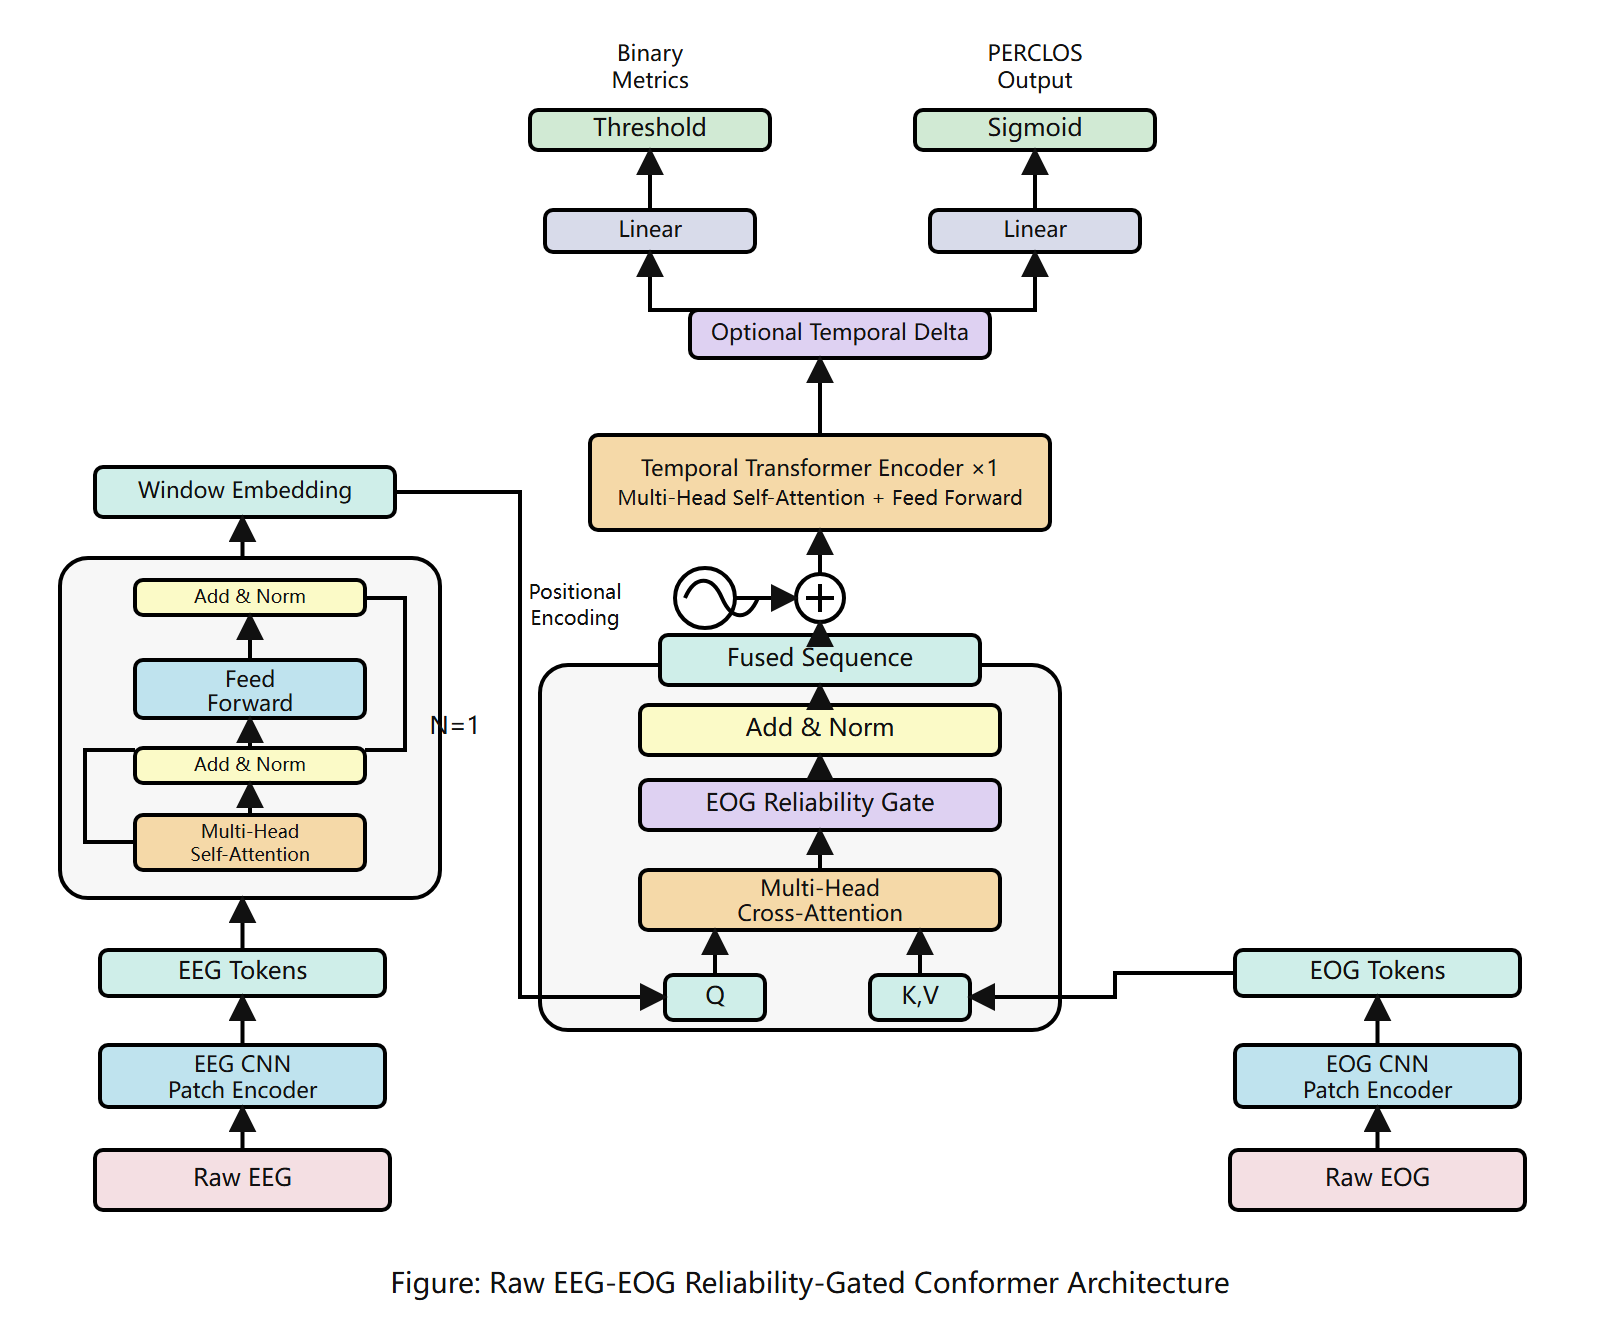
\includegraphics[width=0.92\linewidth]{raw_eeg_eog_reliability_gated_conformer_cn.png}
  \caption{原始 EEG/EOG 可靠性门控融合模型结构。分类指标由 PERCLOS 回归输出阈值化得到，Temporal Delta 仅作为消融模块。}
  \label{fig:arch}
\end{figure}

\section{实验设置}
实验基于 SEED-VIG 数据集。EEG 采样率为 200 Hz，包含 17 个通道；EOG 采样率为 125 Hz，包含 7 个通道。每 8 秒为一个窗口，连续 8 个窗口组成一个 64 秒样本。主结果采用 group-subject 5 折协议，保证测试被试不出现在训练集中。评价指标包括 Accuracy、Macro-F1、Balanced Accuracy、RMSE 和 Pearson 相关系数。训练轮数为 20，batch size 为 4，优化器为 AdamW。

\section{实验结果与分析}
\subsection{主结果}
表~\ref{tab:main} 汇总了严格跨被试协议下的主结果。与传统特征拼接和早期 raw cross-attention 相比，可靠性门控融合显著降低 RMSE 并提高 Pearson。no-delta 版本是当前最适合作为主模型的结果，说明简单时间差分并未带来稳定收益。

\begin{table}[H]
\centering
\caption{主结果（group-subject, binary, 5 折均值）。}
\label{tab:main}
\small
\begin{tabular}{lcccccc}
\toprule
方法 & 训练目标 & Acc$\uparrow$ & F1$\uparrow$ & BalAcc$\uparrow$ & RMSE$\downarrow$ & Pearson$\uparrow$ \\
\midrule
传统特征拼接 & -- & 0.4912 & -- & -- & 0.2563 & 0.5746 \\
Raw EEG/EOG Cross-Attention & regression & 0.7233 & 0.7241 & 0.7332 & 0.1652 & 0.8145 \\
Delta/Gate & regression & 0.8233 & 0.7995 & 0.7977 & 0.1483 & 0.8406 \\
Anchor Residual + Delta & regression & 0.8027 & 0.7894 & 0.7993 & 0.1471 & 0.8398 \\
Reliability-Gated No-Delta & regression & \textbf{0.8263} & \textbf{0.8043} & \textbf{0.8017} & 0.1433 & 0.8508 \\
EOG-only strong baseline & regression & 0.8250 & 0.7883 & 0.7820 & \textbf{0.1432} & \textbf{0.8536} \\
\bottomrule
\end{tabular}
\end{table}

从审稿角度看，本文不应声称多模态融合在所有 clean average 指标上全面超过强基线。更准确的结论是：可靠性门控融合在连续回归指标上达到接近强基线的性能，同时在 F1 和 Balanced Accuracy 上取得更高结果，并且相比传统特征和早期 raw fusion 有明显提升。

\subsection{训练目标消融}
表~\ref{tab:objective} 展示训练目标对结果的影响。CE-only 能直接优化二分类，但会使 RMSE 升至 0.30 以上、Pearson 变为负值，说明它不适合作为连续 PERCLOS 估计的主目标。因此，本文将 regression-only 固定为主方法，classification 与 multitask 仅保留为消融。

\begin{table}[H]
\centering
\caption{训练目标消融（group-subject, binary, 5 折均值）。}
\label{tab:objective}
\small
\begin{tabular}{llccccc}
\toprule
模型 & 目标 & Acc & F1 & BalAcc & RMSE & Pearson \\
\midrule
EOG-only & classification & 0.8261 & 0.8118 & 0.8191 & 0.3070 & -0.4279 \\
Delta-Gate & classification & 0.8080 & 0.7926 & 0.8020 & 0.3105 & -0.7082 \\
EOG-only & regression & 0.8250 & 0.7883 & 0.7820 & 0.1432 & 0.8536 \\
Delta-Gate & regression & 0.8233 & 0.7995 & 0.7977 & 0.1483 & 0.8406 \\
\bottomrule
\end{tabular}
\end{table}

\subsection{划分协议影响}
表~\ref{tab:split} 表明 within-experiment 协议会显著高估泛化能力，而 group-subject 更接近真实跨被试部署场景。本文将 group-subject 作为主结果，有利于避免只在同被试或同实验条件下取得高分。

\begin{table}[H]
\centering
\caption{划分协议影响（EEG+EOG cross-attention, 3-class, 5 折均值）。}
\label{tab:split}
\small
\begin{tabular}{lccccc}
\toprule
协议 & Acc & F1 & BalAcc & RMSE & Pearson \\
\midrule
within-experiment & 0.7732 & 0.7700 & 0.7802 & 0.1320 & 0.8637 \\
group-subject seed0 & 0.7233 & 0.7241 & 0.7332 & 0.1652 & 0.8145 \\
group-subject seed1 & 0.7068 & 0.7098 & 0.7143 & 0.1533 & 0.8370 \\
\bottomrule
\end{tabular}
\end{table}

\subsection{初步鲁棒性分析}
在初步 EOG 退化测试中，部分随机 mask 场景下融合模型仍不够稳定；但在严重 EOG 缺失设置下，融合模型仍保持可用预测能力（EOG 全零场景 RMSE 为 0.3394）。这说明 EEG 分支并非没有作用，但其价值更适合表述为退化保护和困难样本补偿，而不是 clean average 指标上的全面领先。正式投稿前建议将 EOG 退化实验整理为补充表格。

\section{讨论}
本文修订后的核心叙事是“原始 EEG/EOG 的可靠性门控融合与严格跨被试评估”，而不是单纯强调 Delta 模块或追求最高分类准确率。该叙事更能回应审稿人的三个问题：第一，为什么使用回归作为主任务；第二，为什么需要门控而不是直接拼接；第三，在 PERCLOS 与眼动高度相关的数据集中，多模态融合的价值边界在哪里。

本文仍存在局限。首先，当前模型在 clean average 回归指标上未显著超过强基线，因此不能夸大多模态融合的平均性能优势。其次，EOG 部分缺失或随机 mask 场景下的鲁棒性仍需改进。最后，跨被试个体差异仍然明显，未来可进一步引入 subject-invariant 表征学习或自适应校准策略。

\section{结论}
本文提出一种基于原始 EEG/EOG 的可靠性门控融合方法，用于 SEED-VIG 数据集上的驾驶疲劳检测与连续 PERCLOS 警觉度估计。模型通过 EEG-query/EOG-key-value 跨模态注意力读取眼动证据，并使用门控机制控制 EOG 信息注入。实验表明，在严格 group-subject 协议下，no-delta 可靠性门控模型达到 Acc 0.8263、F1 0.8043、RMSE 0.1433 和 Pearson 0.8508，较传统特征和早期 raw fusion 明显提升。消融结果进一步说明，回归目标比 CE-only 更适合 PERCLOS 连续估计，Temporal Delta 当前不宜作为主模块。后续工作将重点完善 EOG 退化鲁棒性分析和跨被试表征对齐。

\begin{thebibliography}{9}
\bibitem{zheng2017}
Zheng W.-L., Lu B.-L. A multimodal approach to estimating vigilance using EEG and forehead EOG. \textit{Journal of Neural Engineering}, 14(2):026017, 2017.

\bibitem{seedvig}
SEED-VIG Dataset. Brain-like Computing and Machine Intelligence Lab, Shanghai Jiao Tong University. \url{https://bcmi.sjtu.edu.cn/home/seed/seed-vig.html}

\bibitem{hmstenet2024}
Tang M., Li P., Zhang H., Deng L., Liu S., Zheng Q., Gao D. HMS-TENet: A hierarchical multi-scale topological enhanced network based on EEG and EOG for driver vigilance estimation. \textit{Biomedical Technology}, 8:92--103, 2024. DOI: 10.1016/j.bmt.2024.10.003.

\bibitem{gelstm2026}
Lan H., Tang M., Ju X., Li M., Hu D. GE-LSTM-Net: A global-enhanced LSTM network with attention for spatiotemporal feature extraction in EEG-based vigilance estimation. \textit{CAAI Artificial Intelligence Research}, 5:9150001, 2026. DOI: 10.26599/AIR.2026.9150001.
\end{thebibliography}

\end{document}
